%% notes-tex/multimodal/043-datasets-primer/sections/6-tensors.tex
%% SOURCE: results/data_shapes_043.json (experiments/043-expression-proteome-morphology/scripts/
%% data_shapes_043.py, slurm job 5902, full pass); the dataset module is
%% experiments/043-expression-proteome-morphology/scripts/dataset_043.py, whose debugger run
%% (six records) is recorded in notes/experiments.043-expression-proteome-morphology.scripts.dataset_043.md.

\section{Data as tensors\secstatus{todo}}
\label{sec:tensors}

Figure~\ref{fig:data-flow} follows a record from the store to a batch, and
Table~\ref{tab:shapes} gives each dataset's shape from a full pass over the 173{,}617
records. A record is a pair of experiment and experiment reference; its genotype becomes
a set of marked genes on the 6{,}607-gene index $G$ of \file{gene_set.json}, its phenotype
a vector $y$ over $G$ with \texttt{NaN} where a gene is not measured, and its environment,
dataset and experiment type become integer tokens.

%% SOURCE: notes/experiments.043-expression-proteome-morphology.mermaid.data-flow.md, rendered by
%% notes/assets/publish/scripts/mermaid_pdf.sh, copied to figures/ by `make diagrams`
\begin{figure}[htbp]\centering
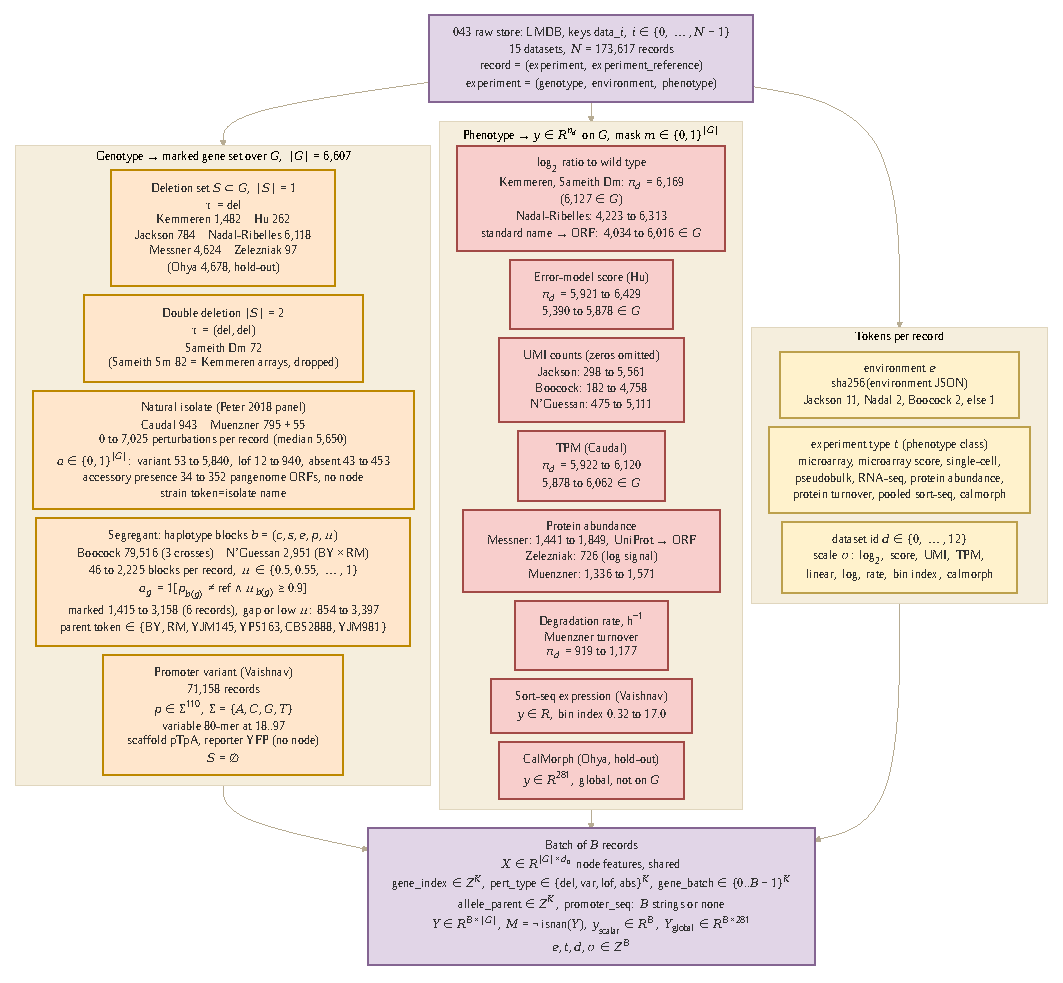
\includegraphics[width=\textwidth]{figures/mermaid-data-flow.pdf}\par\vspace{2pt}
\caption[]{\textbf{A record of the store becomes a marked gene set, a masked label vector
and four tokens.} Left, the five genotype classes and the counts each marks; middle, the
nine released label scales with the number of label keys per record and how many of them
fall on $G$; right, the environment, experiment-type and dataset tokens; bottom, the batch
the collate function returns. Rendered 212 mm wide and placed at 180 mm, a scale of 0.85.}
\label{fig:data-flow}
\end{figure}
%% Generated by notes/assets/publish/scripts/mermaid_pdf.sh from
%% notes/experiments.043-expression-proteome-morphology.mermaid.data-flow.md

\notesec{What the dataset module returns}
Per sample, \file{dataset_043.py} returns the marked genes as indices on $G$
(\file{gene_index}), a change type per marked gene (\file{pert_type}), the allele parent
per marked gene for the segregants (\file{allele_parent}), the promoter sequence and
scaffold for Vaishnav, the environment, dataset and experiment-type ids, the label scale
(\file{y_scale}), the label $y\in\mathbb{R}^{6{,}607}$, one scalar for Vaishnav and the
281 CalMorph features for Ohya. The collate function concatenates the marked genes with a
batch vector and stacks $y$ into a $B\times 6{,}607$ tensor with its measured mask. A
mixed batch of one record per dataset, 15 rows, carries 21{,}728 marked genes, 21{,}713
of them from the five isolate and segregant rows (the six-record debugger run).

\notesec{Three shapes that bear on the design}
The isolate and segregant rows are dense: a Caudal isolate marks 4{,}952 to 5{,}995 of
6{,}607 genes and a segregant 1{,}415 to 3{,}158 under the definite rule, against one
for a deletion, so the perturbation operator sees three orders of magnitude of marked-set
size across datasets (counts on the debugger records). The definite rule leaves gaps: on
the six debugger records 697 to 2{,}693 genes fall between blocks and 157 to 704 under a
block below posterior 0.9. Two label-key maps run at read time: Nadal-Ribelles keys are
standard names (1{,}441 of 6{,}796 on $G$ by raw name, 6{,}325 after the map) and Messner
keys are UniProt accessions (0 of 1{,}850 by raw name, 1{,}850 after). A key with no
position on $G$ is counted per sample and dropped from $y$, never guessed.

%% SOURCE: experiments/043-expression-proteome-morphology/scripts/primer_043_tables.py
%% -> tables/t12-shapes-rows.tex (results/data_shapes_043.json)
\begin{landscape}
\scriptsize
\setlength{\tabcolsep}{3pt}
\begin{longtable}{>{\raggedright\arraybackslash}p{24mm}>{\raggedright\arraybackslash}p{24mm}>{\raggedleft\arraybackslash}p{12mm}>{\raggedright\arraybackslash}p{24mm}>{\raggedleft\arraybackslash}p{20mm}>{\raggedright\arraybackslash}p{31mm}>{\raggedleft\arraybackslash}p{19mm}>{\raggedleft\arraybackslash}p{23mm}>{\raggedleft\arraybackslash}p{23mm}>{\raggedleft\arraybackslash}p{18mm}}
\caption[]{\textbf{Every dataset of the store as tensors.} One row per dataset, from a
full pass over the raw store (\file{data_shapes_043.py}, slurm job 5902). Perturbations
per record count the released perturbation list (a segregant has none; its genotype is a
list of haplotype blocks). Label values are the finite minimum and maximum over a sample
of each dataset's values, on the released scale. Label keys on $G$ count the keys that
land on the 6{,}607-gene index after the read-time maps. Where a cell shows one number,
minimum, median and maximum are equal; otherwise it reads median (minimum to
maximum).}\label{tab:shapes}\\
\toprule
Dataset & Role in the plan & Records, n & Genotype class (records) & Perturbations per record & Label key, graph level & Label values, min to max & Label keys per record & Label keys on $G$ per record & Environments, n \\
\midrule
\endfirsthead
\toprule
Dataset & Role in the plan & Records, n & Genotype class (records) & Perturbations per record & Label key, graph level & Label values, min to max & Label keys per record & Label keys on $G$ per record & Environments, n \\
\midrule
\endhead
%% GENERATED by experiments/043-expression-proteome-morphology/scripts/primer_043_tables.py
%% SOURCE: results/data_shapes_043.json (data_shapes_043.py, slurm job 5902, mode full). Do not edit by hand.
Kemmeren 2014 & train; split A holds out 10\% of genes & 1{,}482 & Genotype & 1 & \texttt{expression\_log2\_ratio}, node & $-$6.72 to 6.17 & 6{,}169 & 6{,}127 & 1 \\
Sameith 2015 Sm & dropped: Kemmeren's arrays & 82 & Genotype & 1 & \texttt{expression\_log2\_ratio}, node & $-$4.31 to 5.23 & 6{,}169 & 6{,}127 & 1 \\
Sameith 2015 Dm & split B: every double held out & 72 & Genotype & 2 & \texttt{expression\_log2\_ratio}, node & $-$6.25 to 4.8 & 6{,}169 & 6{,}127 & 1 \\
Hu 2007 & train & 262 & Genotype & 1 & \texttt{expression\_score}, node & $-$8.35 to 8.05 & 6{,}381 (5{,}921 to 6{,}429) & 5{,}832 (5{,}390 to 5{,}878) & 1 \\
Jackson 2020 & train & 784 & Genotype & 1 & \texttt{umi\_count}, node & 1 to 21{,}655 & 4{,}028 (298 to 5{,}561) & 4{,}009 (298 to 5{,}501) & 11 \\
Nadal-Ribelles 2025 & train & 6{,}118 & Genotype & 1 & \texttt{expression\_log2\_ratio}, node & $-$33 to 32.9 & 5{,}866 (4{,}223 to 6{,}313) & 5{,}665 (4{,}034 to 6{,}016) & 2 \\
Messner 2023 & train & 4{,}624 & Genotype & 1 & \texttt{protein\_abundance}, node & 0.0313 to 393{,}221 & 1{,}819 (1{,}441 to 1{,}849) & 1{,}819 (1{,}441 to 1{,}849) & 1 \\
Zelezniak 2018 & train & 97 & Genotype & 1 & \texttt{protein\_abundance}, node & 1.62 to 11.2 & 726 & 726 & 1 \\
Ohya 2005 & probe only, frozen latent & 4{,}678 & Genotype & 1 & \texttt{calmorph}, global & 0 to 56{,}974 & 281 & none, features not genes & 1 \\
Caudal 2024 & train; split C isolates held out & 943 & Genotype + natural isolate & 5{,}662 (195 to 7{,}025) & \texttt{expression\_tpm}, node & 0 to 88{,}829 & 6{,}050 (5{,}922 to 6{,}120) & 6{,}006 (5{,}878 to 6{,}062) & 1 \\
Muenzner 2024 protein & train; split C holds out a fifth of isolates & 795 & Genotype + natural isolate (794); Genotype (1) & 5{,}628 (0 to 7{,}025) & \texttt{protein\_abundance}, node & 0.0906 to 181{,}277 & 1{,}540 (1{,}336 to 1{,}571) & 1{,}540 (1{,}336 to 1{,}571) & 1 \\
Muenzner 2024 turnover & train; split C isolates held out & 55 & Genotype + natural isolate & 5{,}662 (4{,}903 to 6{,}430) & \texttt{degradation\_rate}, node & 0.0169 to 2.44 & 1{,}055 (919 to 1{,}177) & 1{,}055 (919 to 1{,}177) & 1 \\
Boocock 2025 & train & 79{,}516 & SegregantGenotype & 0 & \texttt{umi\_count}, node & 1 to 2{,}301 & 962 (182 to 4{,}758) & 962 (182 to 4{,}758) & 2 \\
N'Guessan 2025 & train & 2{,}951 & SegregantGenotype & 0 & \texttt{umi\_count}, node & 1 to 12{,}339 & 2{,}592 (475 to 5{,}111) & 2{,}591 (475 to 5{,}109) & 1 \\
Vaishnav 2022 & train, promoter signal & 71{,}158 & Genotype & 1 & \texttt{expression\_level}, node & 0.321 to 17 & 1 & none, one scalar & 1 \\
\midrule
Total & & 173{,}617 & & & & & & 6{,}607 genes on the index & \\
\bottomrule

\end{longtable}
\end{landscape}
